%******************************************************************************%
%                                                                              %
%                  JavaScript.en.tex for LaTeX                                 %
%                  Created on : Tue Mar 10 13:27:28 2015                       %
%                  Made by : Don Stolz <dstolz@student.42.us.org>              %
%                                                                              %
%******************************************************************************%

\documentclass{42-en}


%******************************************************************************%
%                                                                              %
%                                    Header                                    %
%                                                                              %
%******************************************************************************%
\begin{document}
\title{MongoDB}
\member{Donald Stolz}{dstolz@student.42.us.org}
\summary {
 Setup a MongoDB cloud account and cluster. 
}
\maketitle

\tableofcontents

%******************************************************************************%
%                                                                              %
%                                 Introduction                                 %
%                                                                              %
%******************************************************************************%
\chapter{Introduction}

When building applications, whether it's a social media app or a todo list, different types of data often need to be stored. MongoDB is one versatile option for storing data. It's an open source, non-relational database that uses a document model allowing for flexibility in the structuring of your data. It’s also highly scalable, dynamic, and the leading NoSQL database. \\

Additional Resources:
\begin{itemize}\itemsep1pt
\item \href{https://www.mongodb.com/what-is-mongodb}{What is MongoDB}
\item \href{https://medium.com/xplenty-blog/the-sql-vs-nosql-difference-mysql-vs-mongodb-32c9980e67b2}{NoSQL vs. SQL, what's the difference?}
\item \href{https://www.upwork.com/hiring/data/should-you-use-mongodb-a-look-at-the-leading-nosql-database}{Should you use MongoDB?}
\end{itemize}

%******************************************************************************%
%                                                                              %
%                                  Instructions                                %
%                                                                              %
%******************************************************************************%
\chapter{Instructions}

First head to \href{https://www.mongodb.com/}{https://www.mongodb.com/}

\begin{figure}[H]
    \begin{center}
        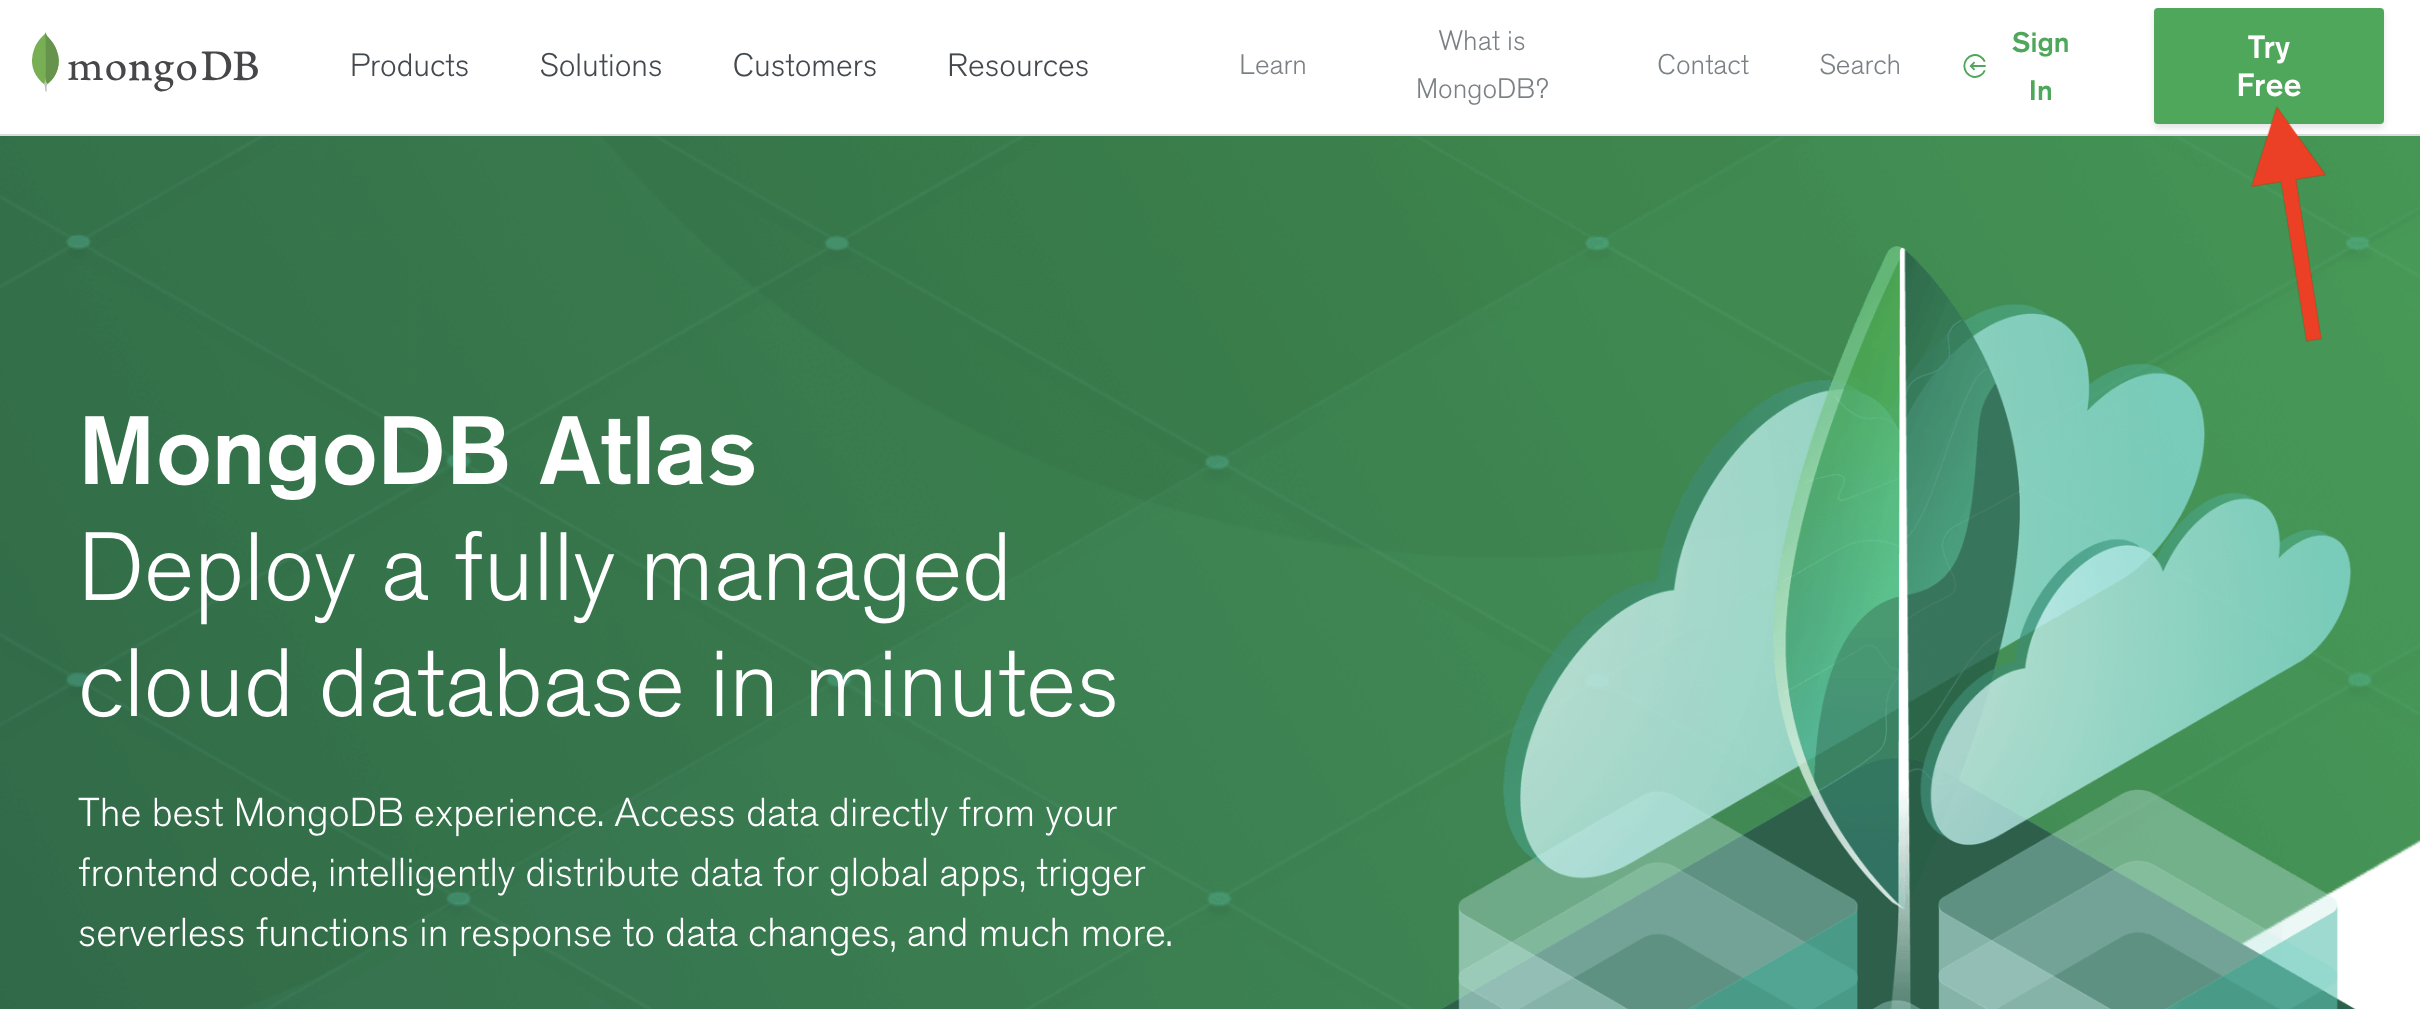
\includegraphics[width=14cm]{WEB/mongo_0.png}
    \end{center}
\end{figure}

Fill out the simple form to create an account
\begin{figure}[H]
    \begin{center}
        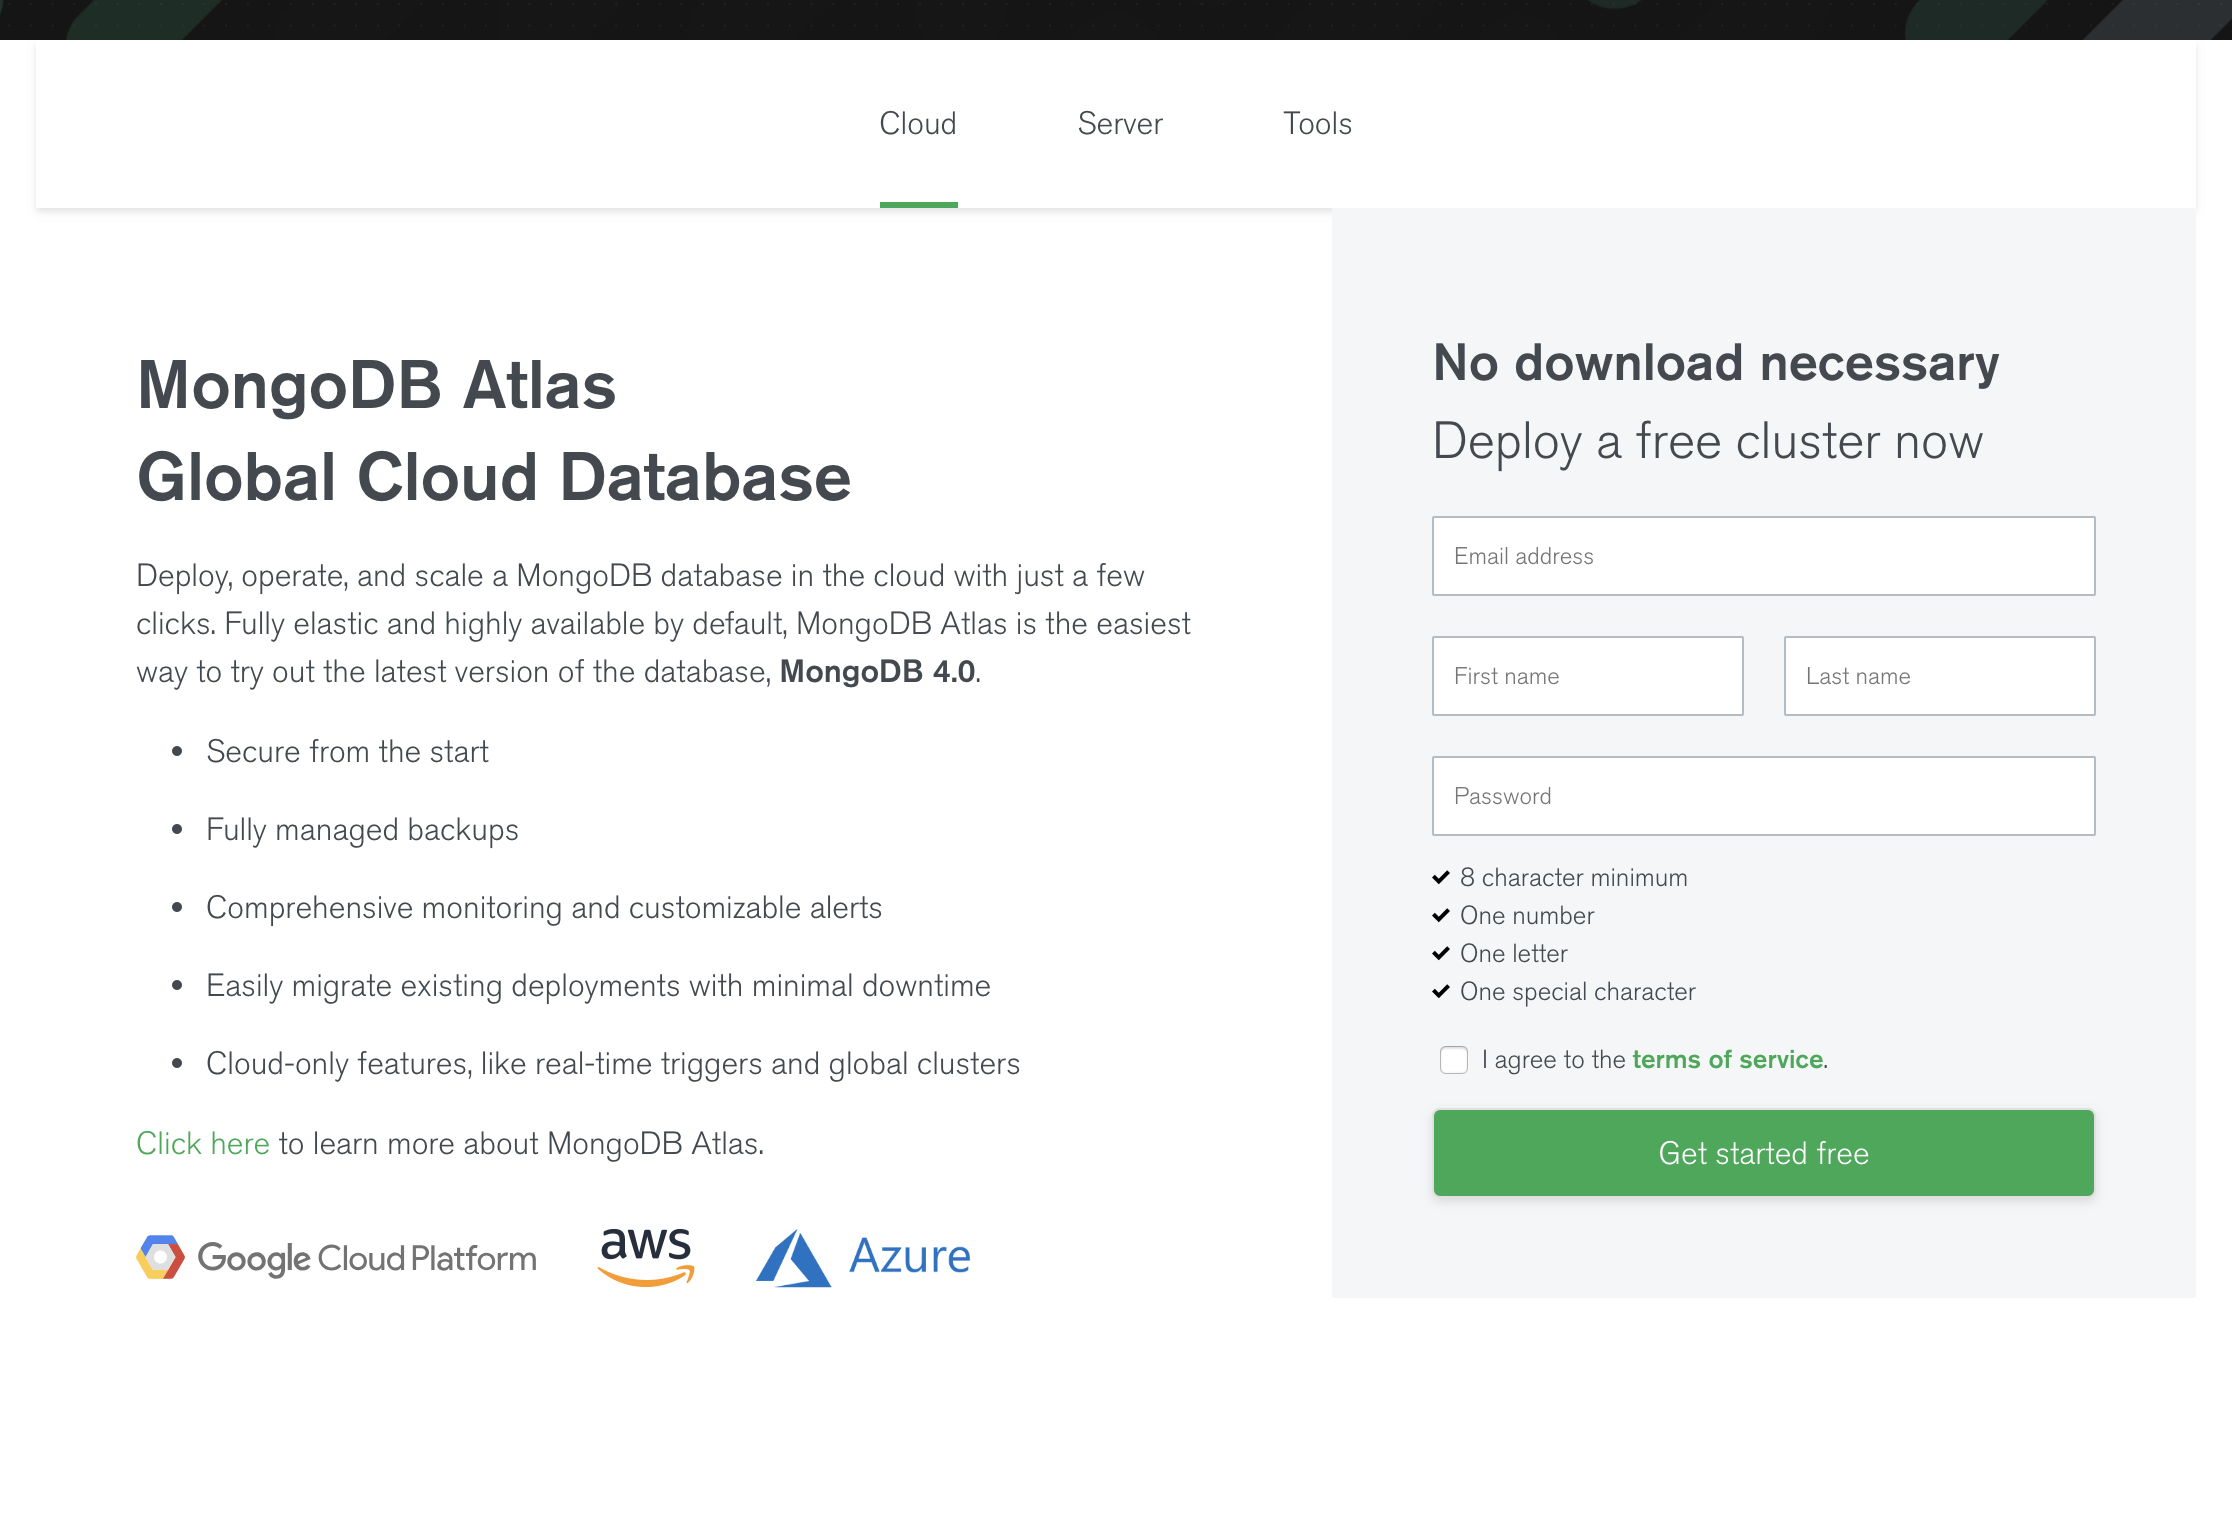
\includegraphics[width=14cm]{WEB/mongo_1.png}
    \end{center}
\end{figure}

\newpage
Once you start creating a new cluster the only piece of the form you should change is the Cluster Name, at the bottom
\begin{figure}[H]
    \begin{center}
        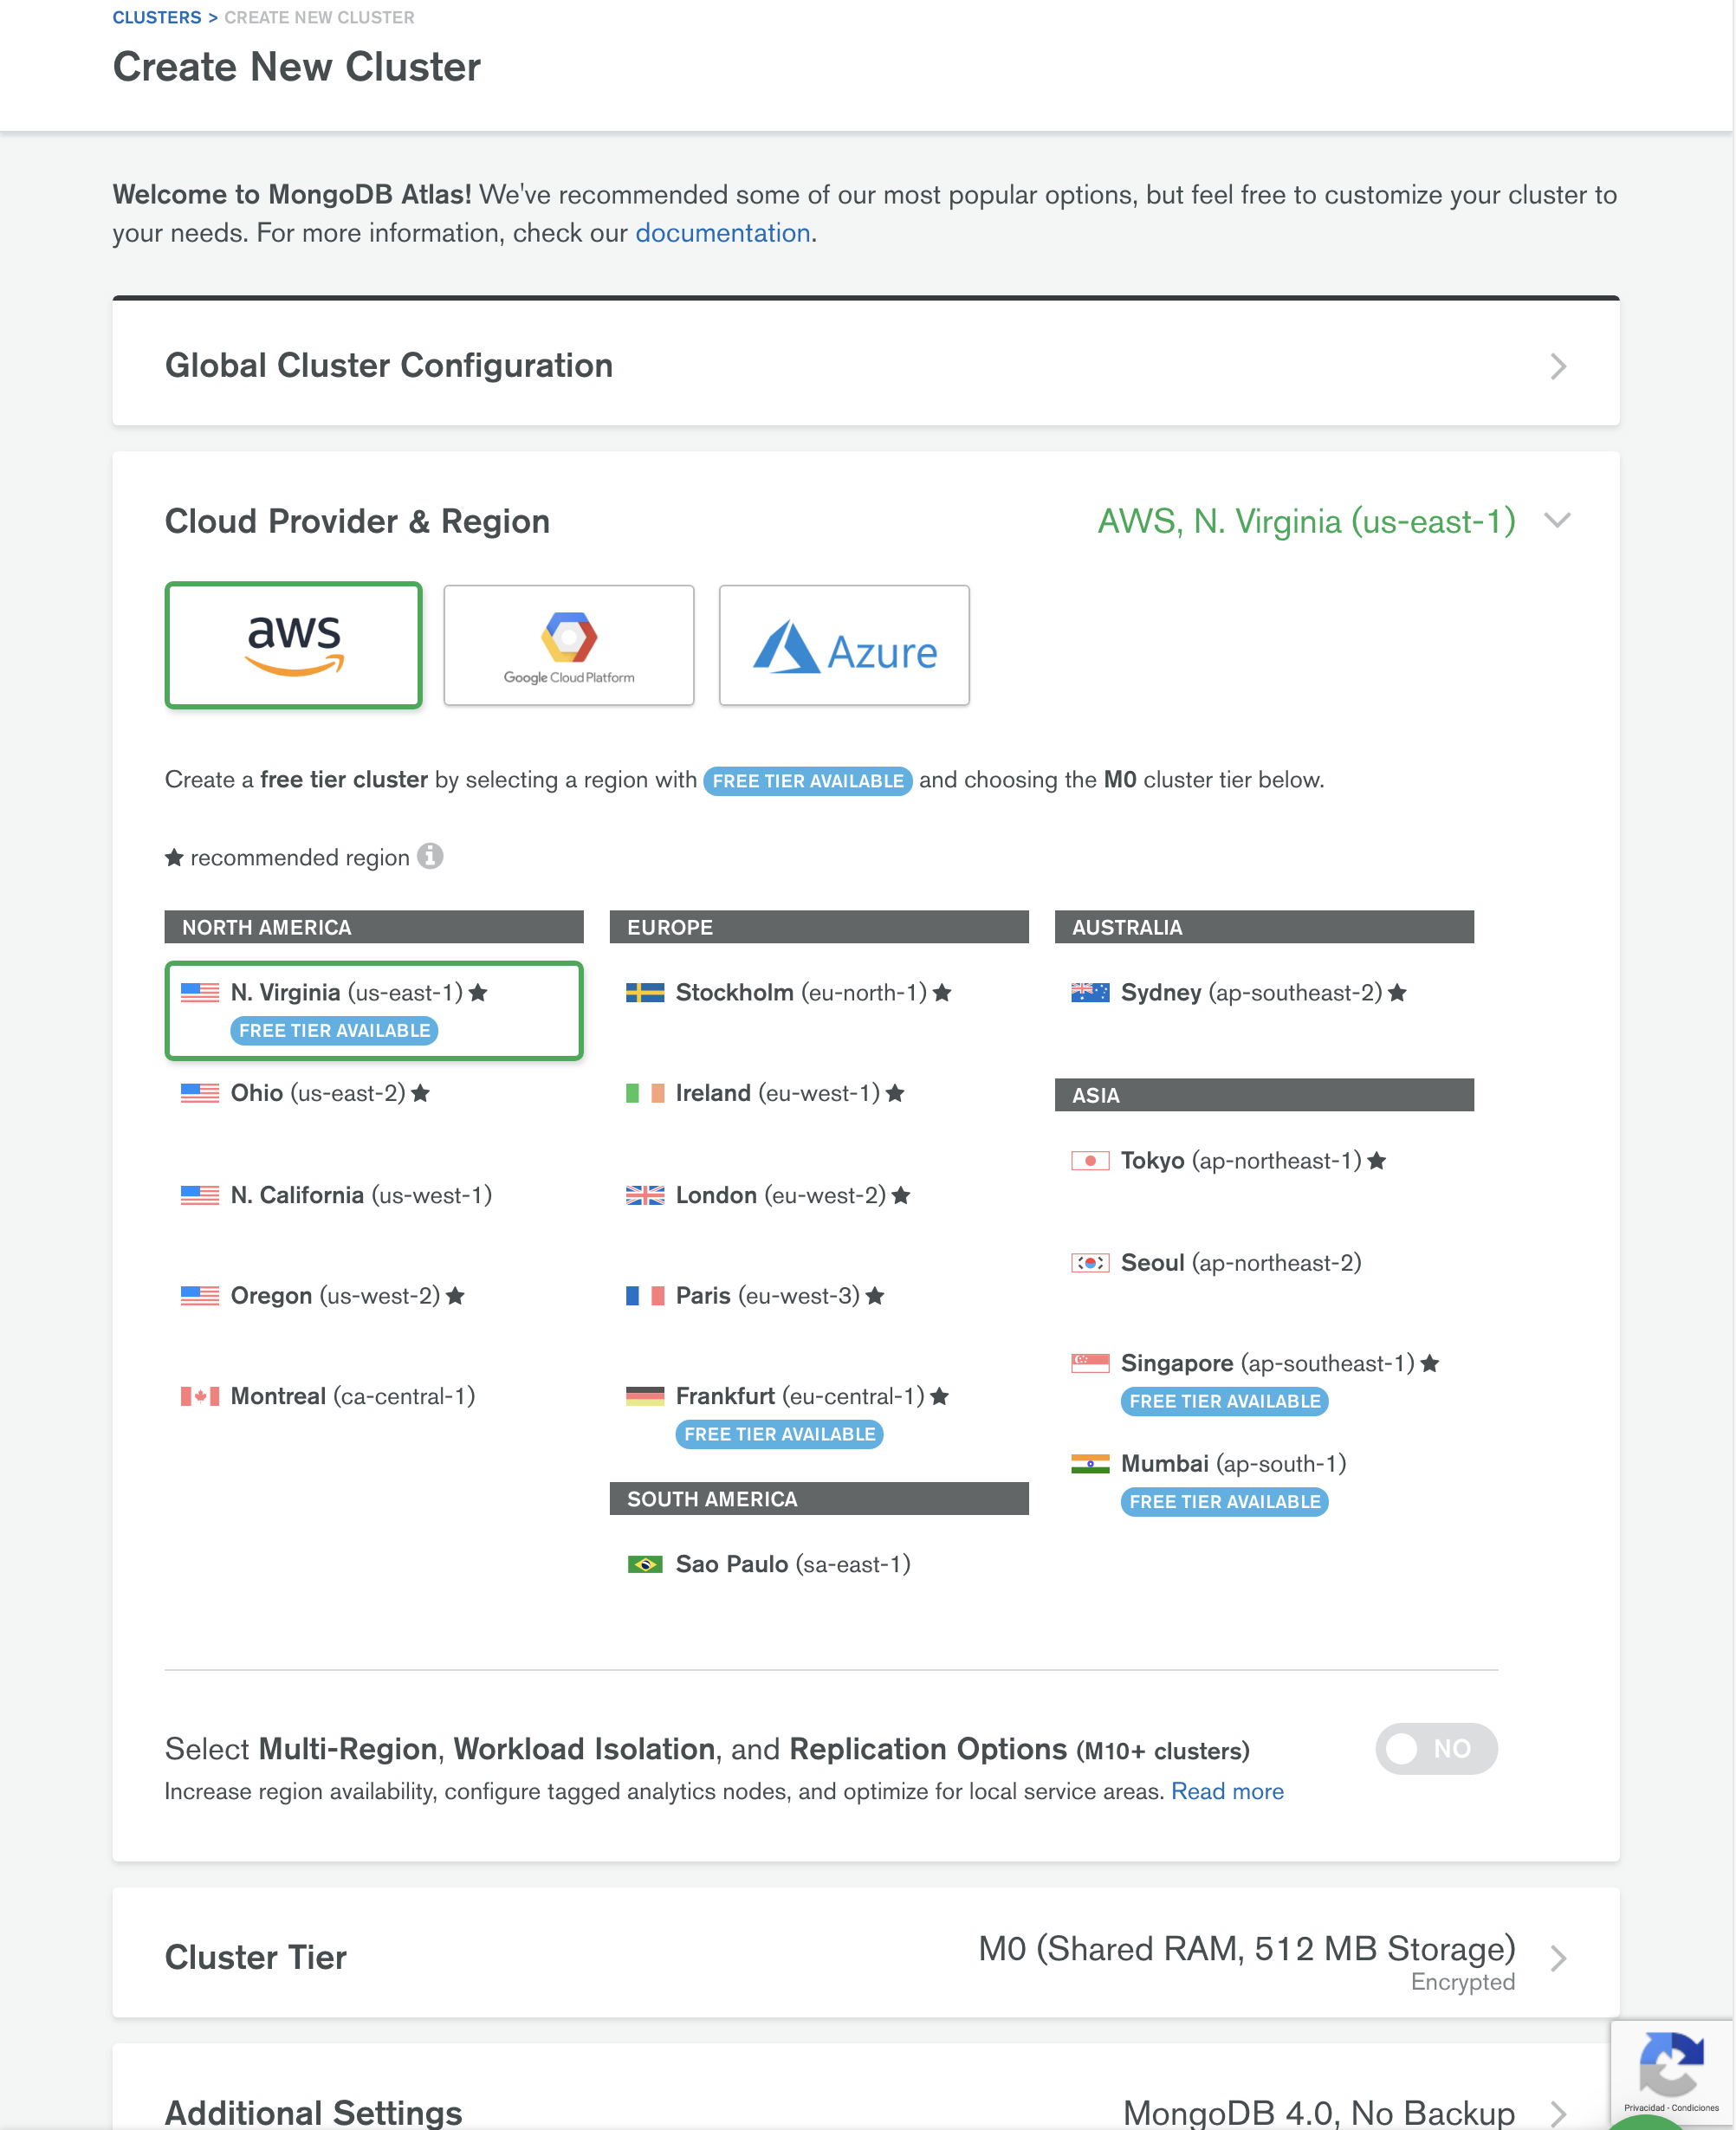
\includegraphics[width=12cm]{WEB/mongo_2.png}
    \end{center}
\end{figure}

\begin{figure}[H]
    \begin{center}
        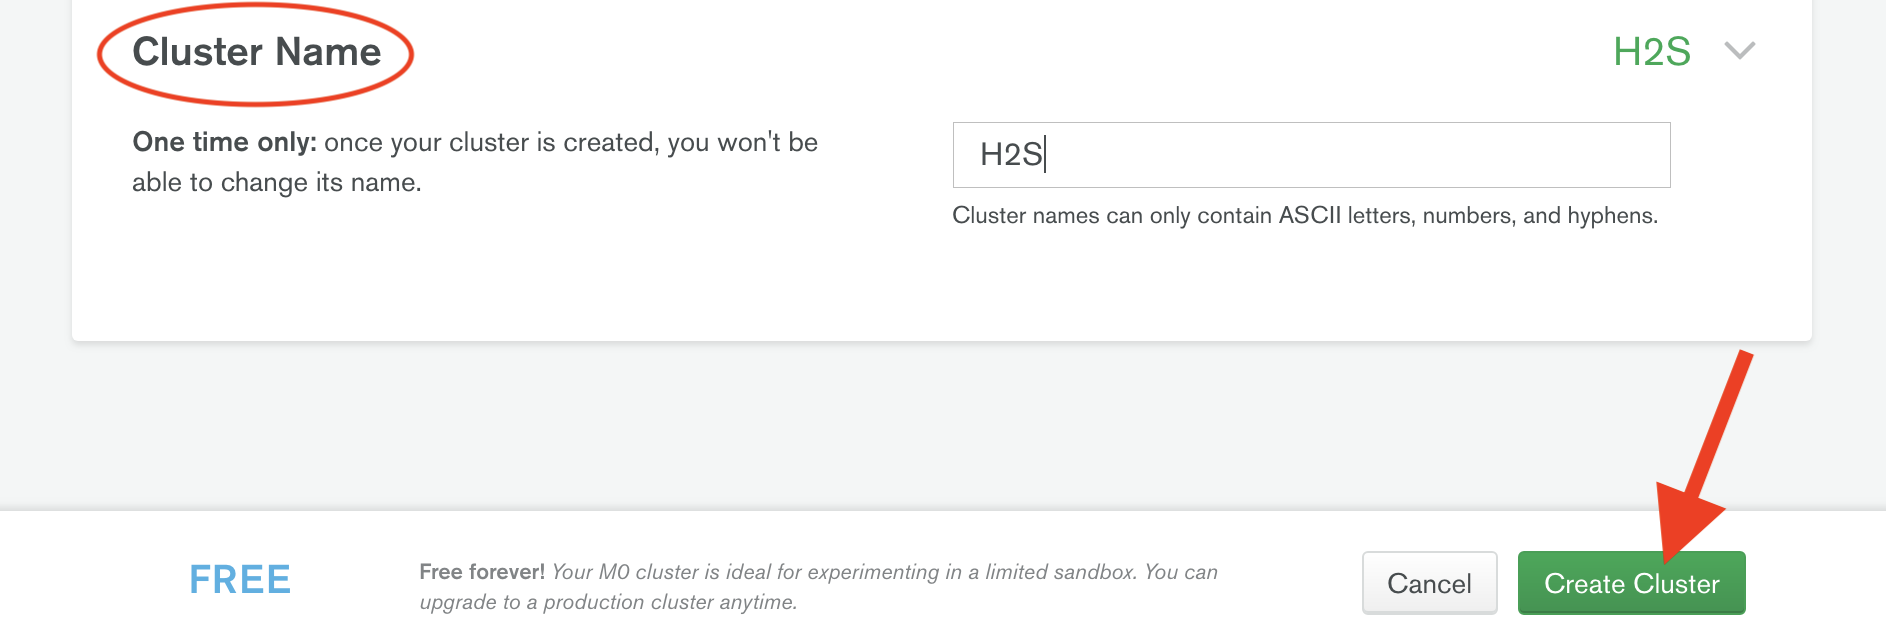
\includegraphics[width=14cm]{WEB/mongo_3.png}
    \end{center}
\end{figure}

\newpage
Now create a database user. This will allow you to connect to your cluster as a specific user. You can set up different permissions and authentication credentials for different users (for example if someone is allowed to read the data in your database but not modify it).
\begin{figure}[H]
    \begin{center}
        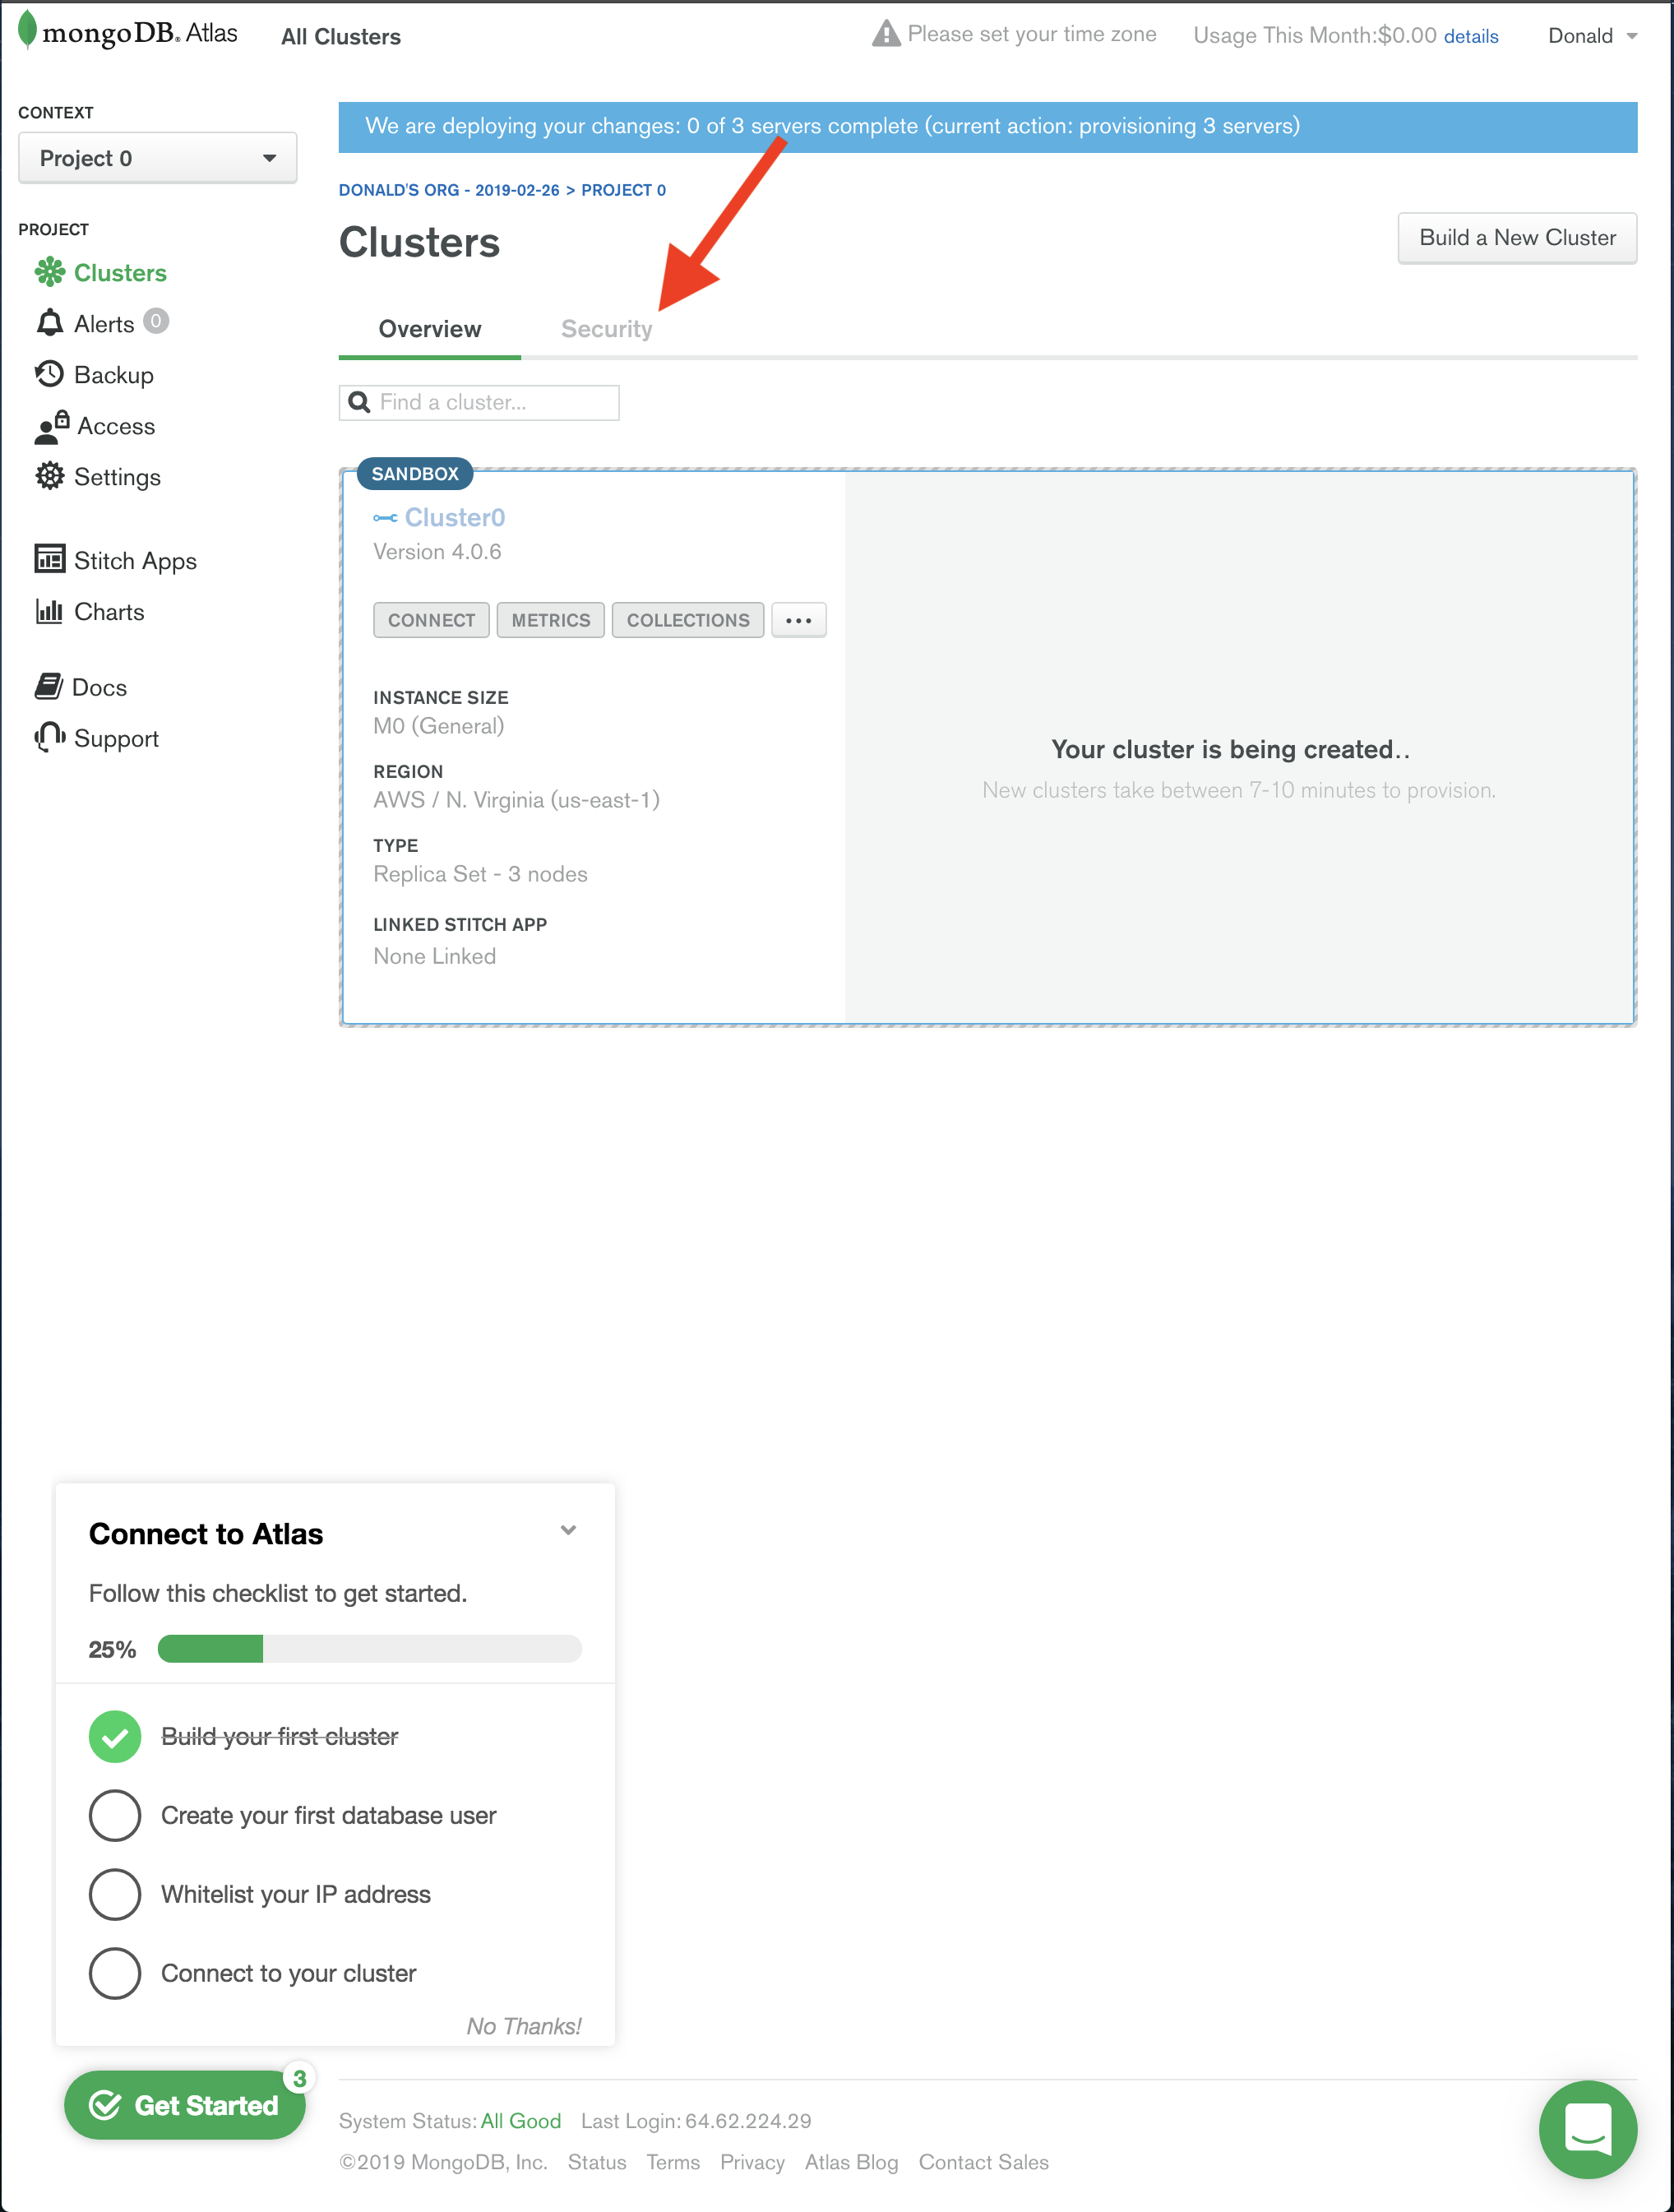
\includegraphics[width=14cm]{WEB/mongo_4.png}
    \end{center}
\end{figure}

\begin{figure}[H]
    \begin{center}
        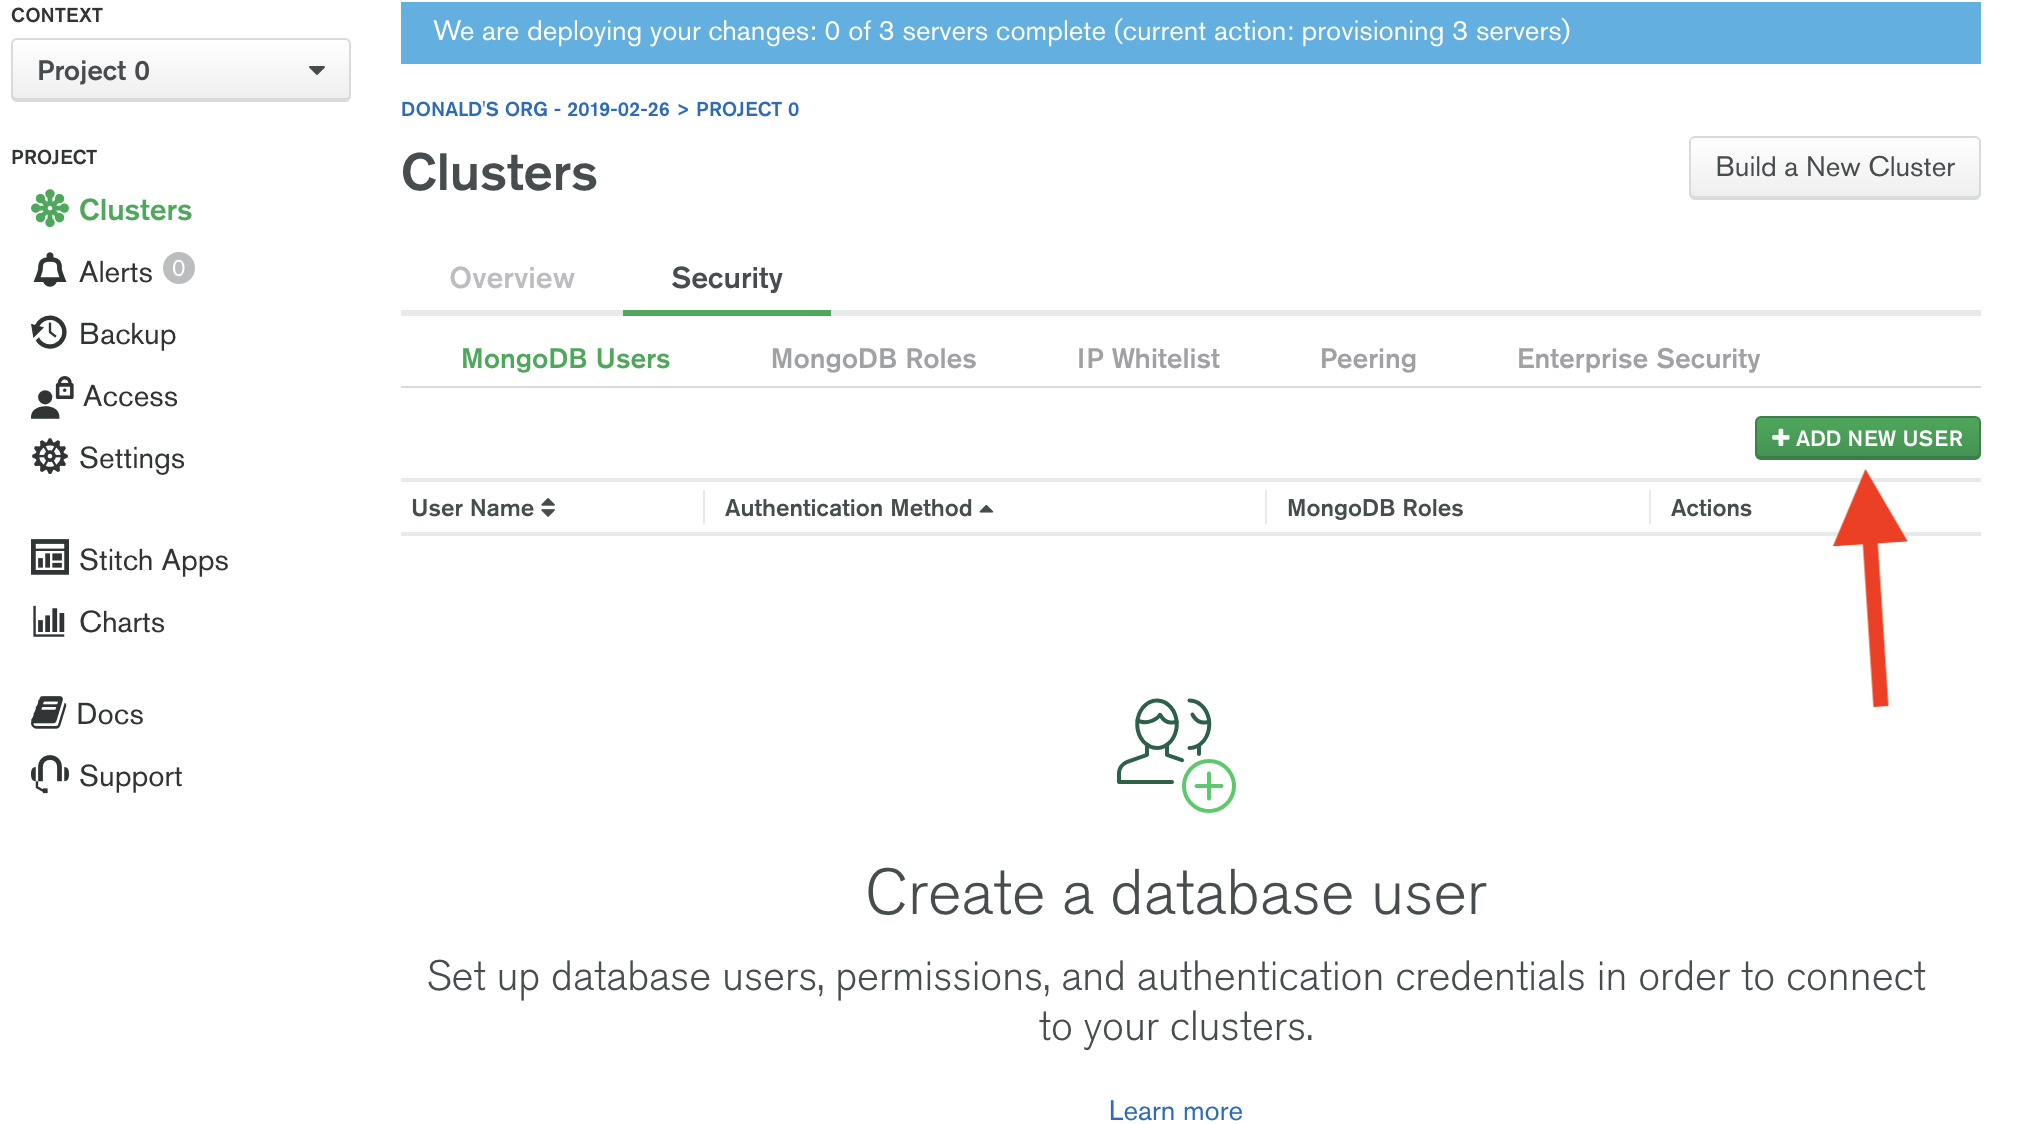
\includegraphics[width=14cm]{WEB/mongo_5.png}
    \end{center}
\end{figure}

\begin{figure}[H]
    \begin{center}
        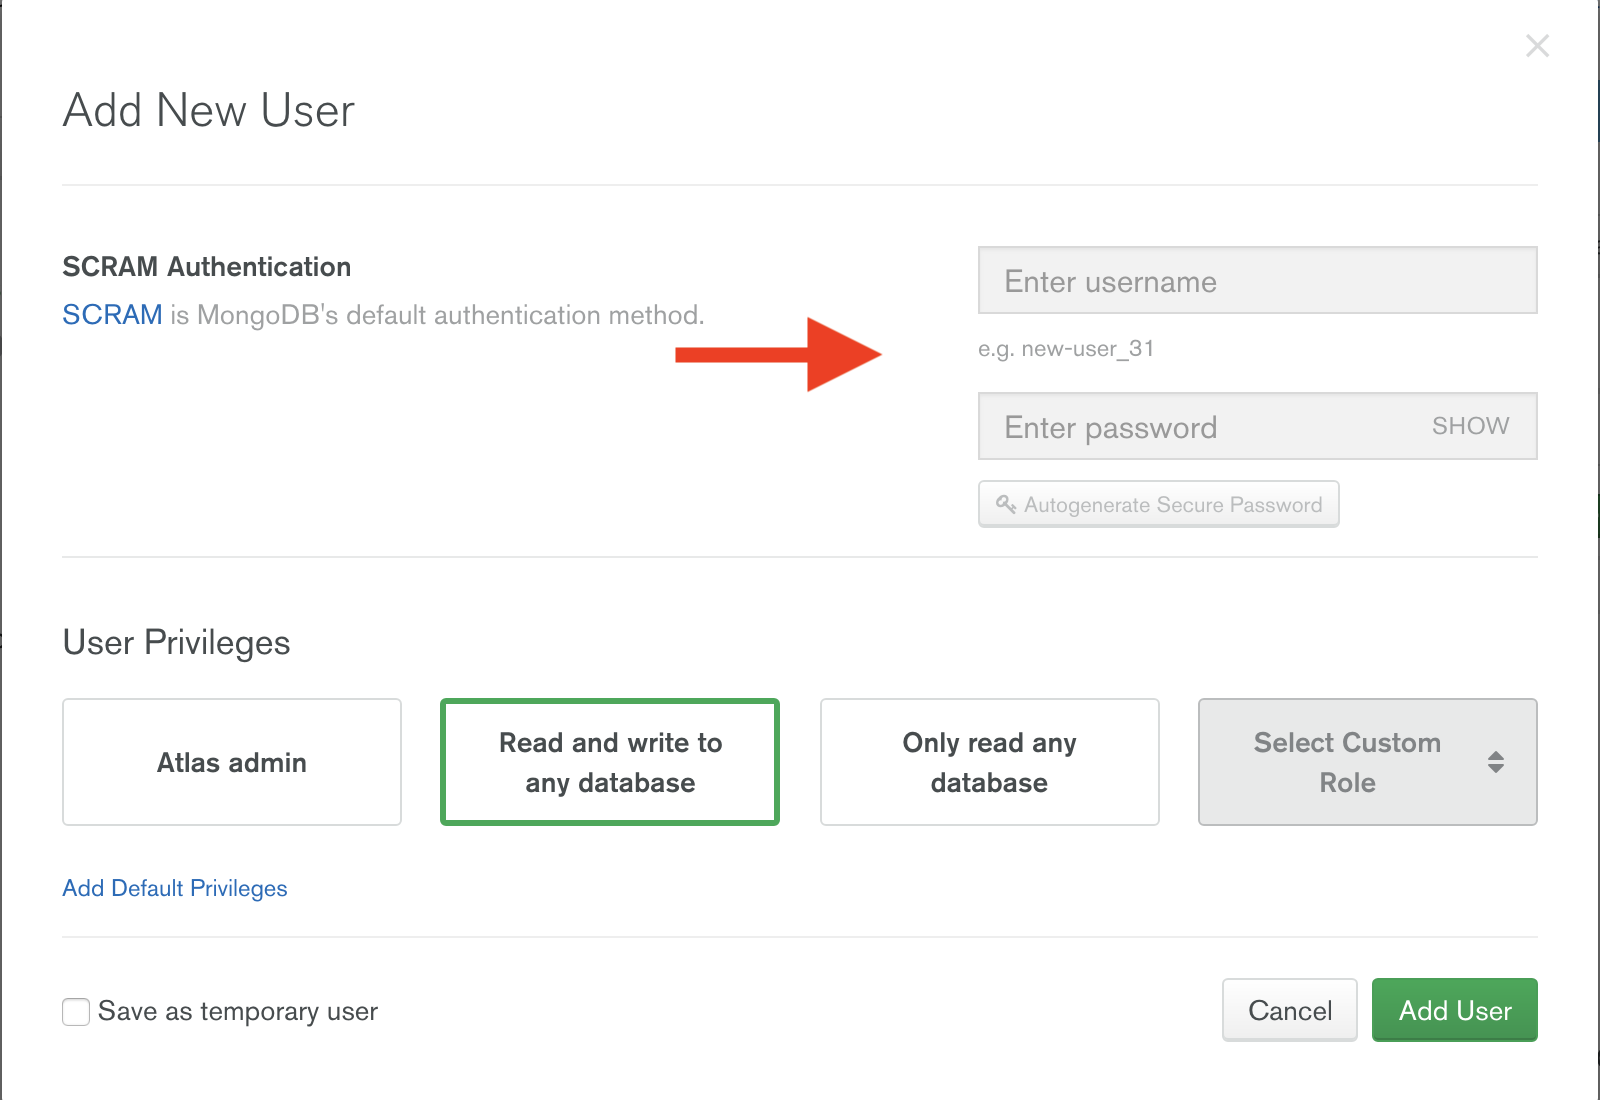
\includegraphics[width=14cm]{WEB/mongo_6.png}
    \end{center}
\end{figure}

\begin{figure}[H]
    \begin{center}
        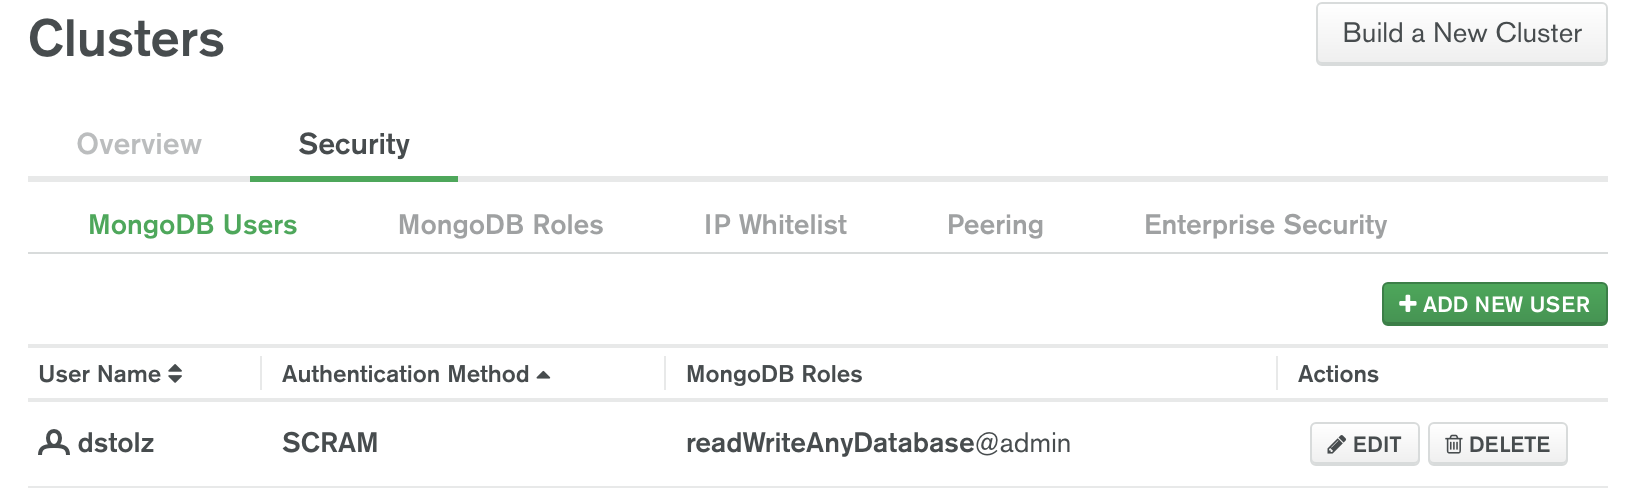
\includegraphics[width=14cm]{WEB/mongo_7.png}
    \end{center}
\end{figure}

\newpage
After creating a user you will need to whitelist your IP address
\begin{figure}[H]
    \begin{center}
        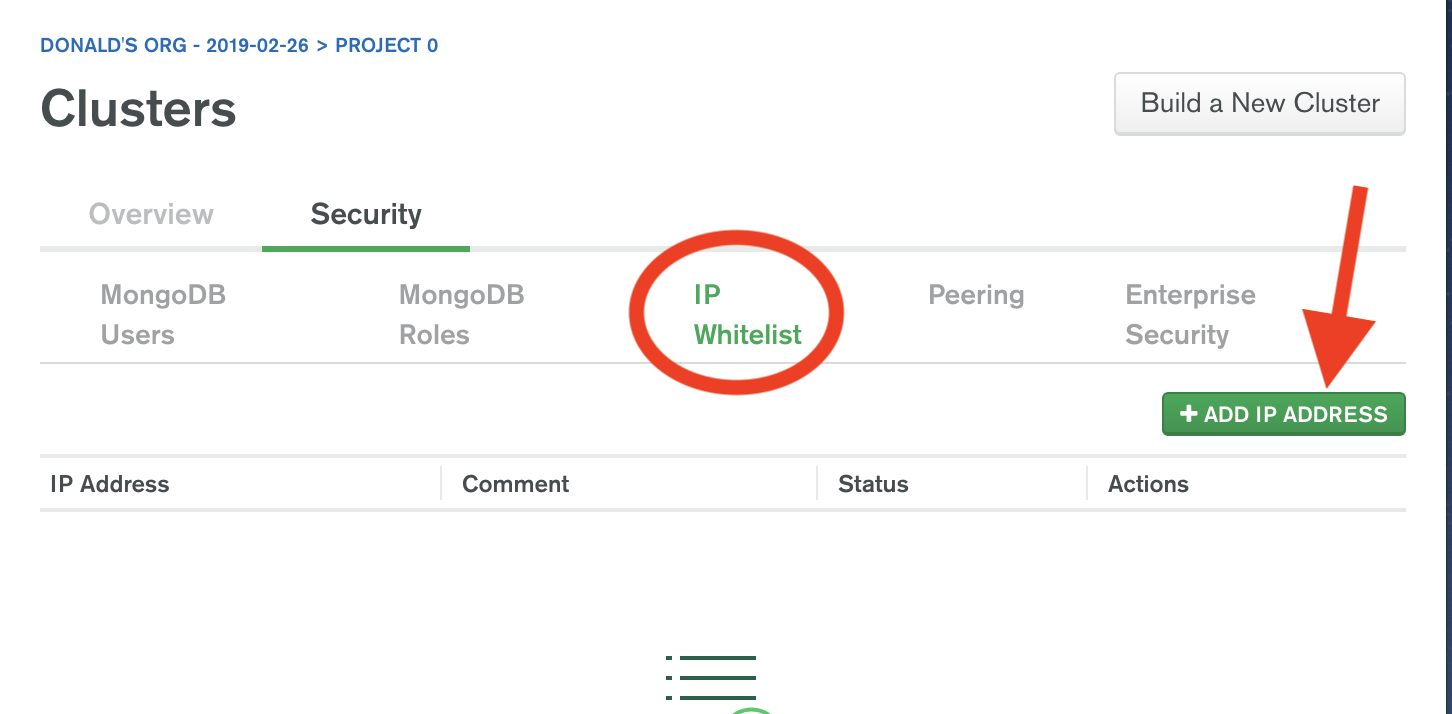
\includegraphics[width=14cm]{WEB/mongo_8.png}
    \end{center}
\end{figure}

\begin{figure}[H]
    \begin{center}
        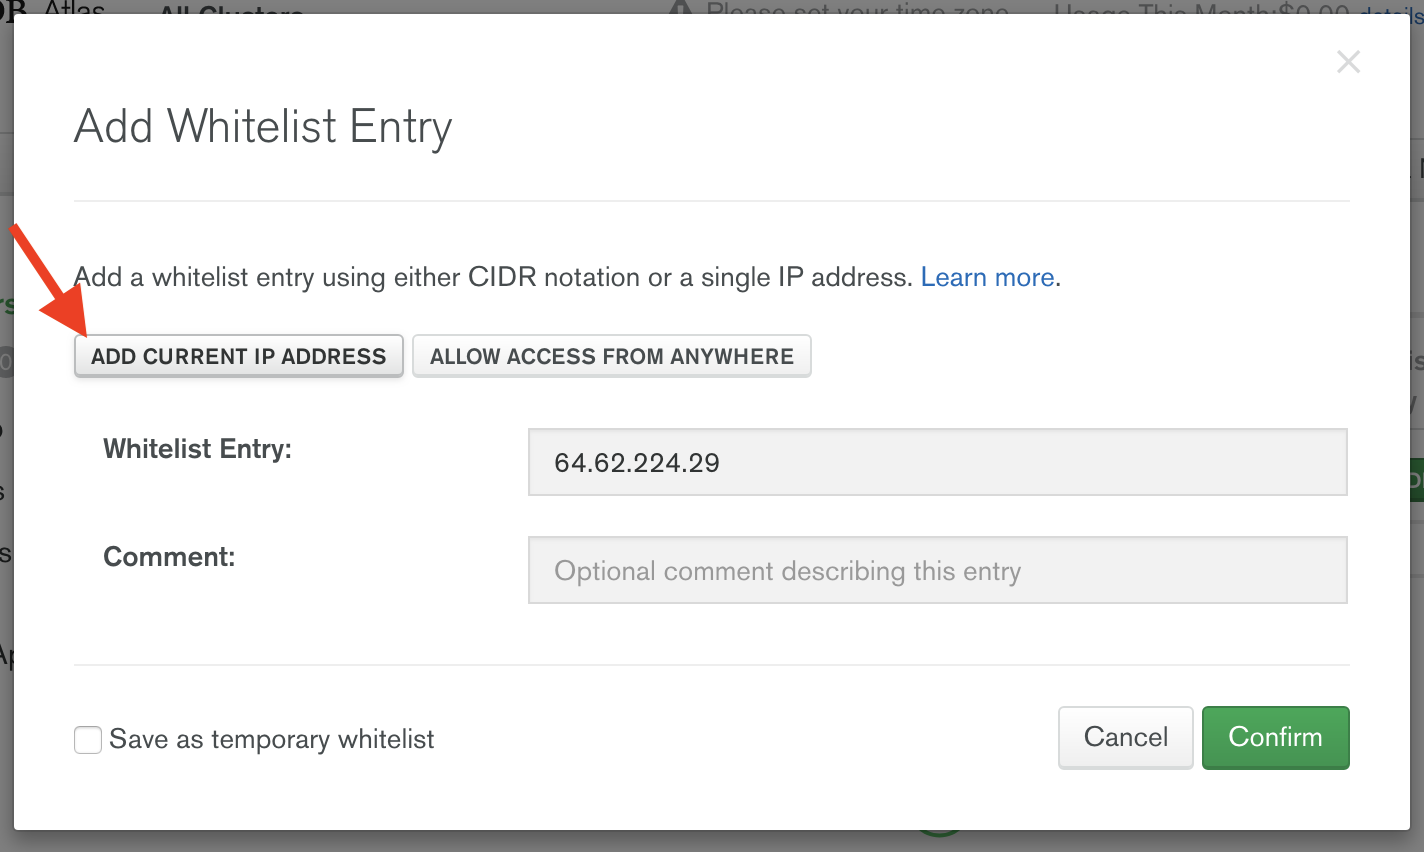
\includegraphics[width=14cm]{WEB/mongo_9.png}
    \end{center}
\end{figure}

\newpage
Once we have a user and our IP address is whitelisted we can get the address for connecting our app.
\begin{figure}[H]
    \begin{center}
        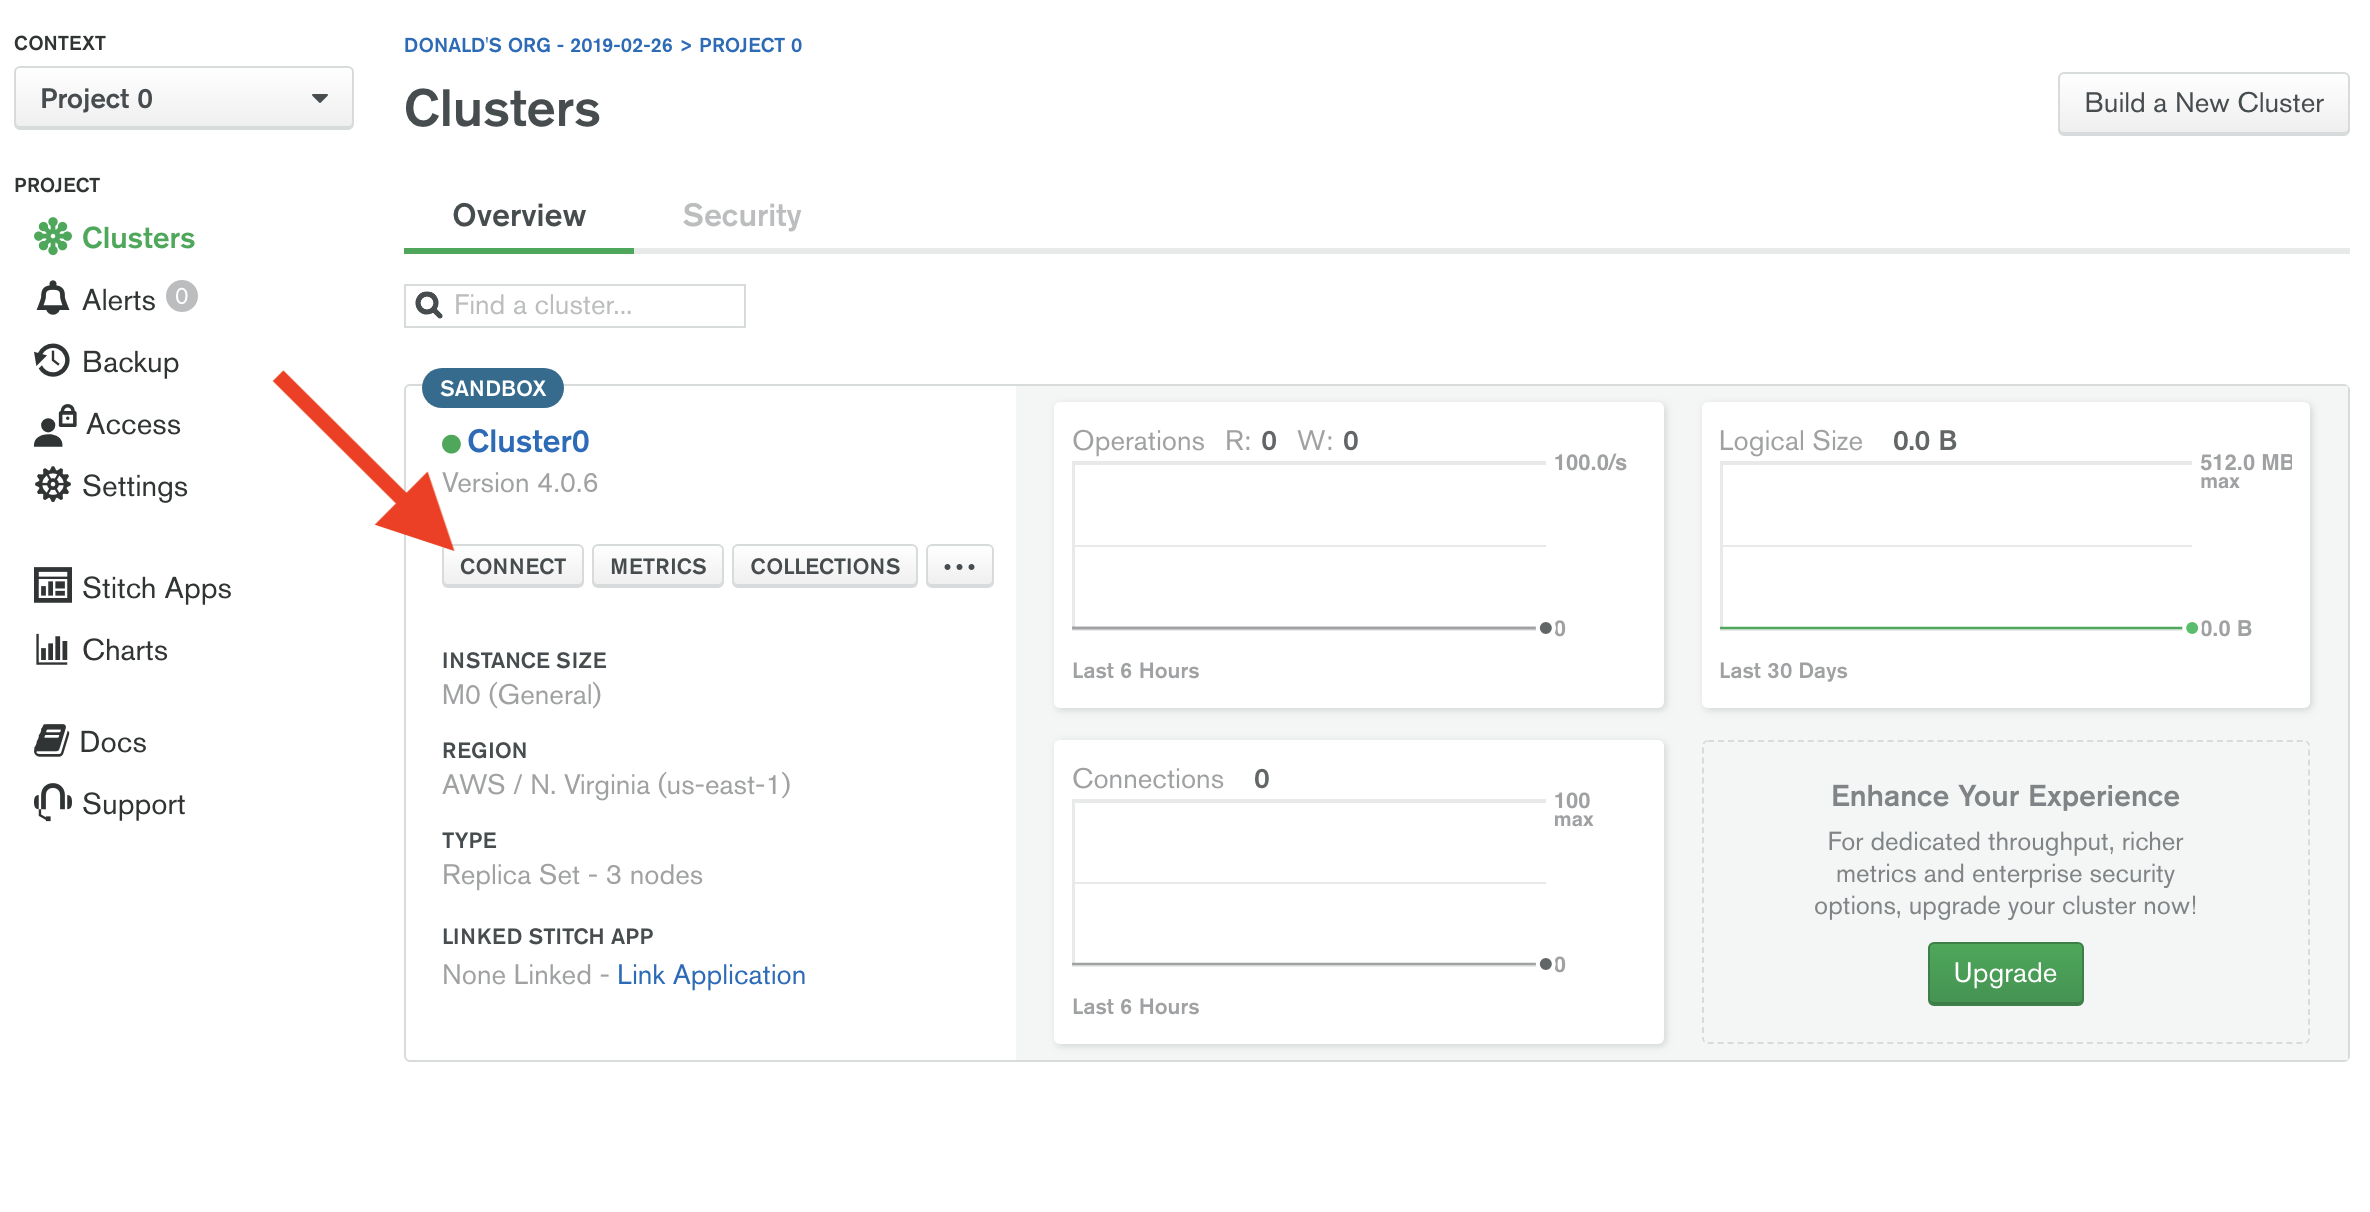
\includegraphics[width=14cm]{WEB/mongo_10.png}
    \end{center}
\end{figure}

\begin{figure}[H]
    \begin{center}
        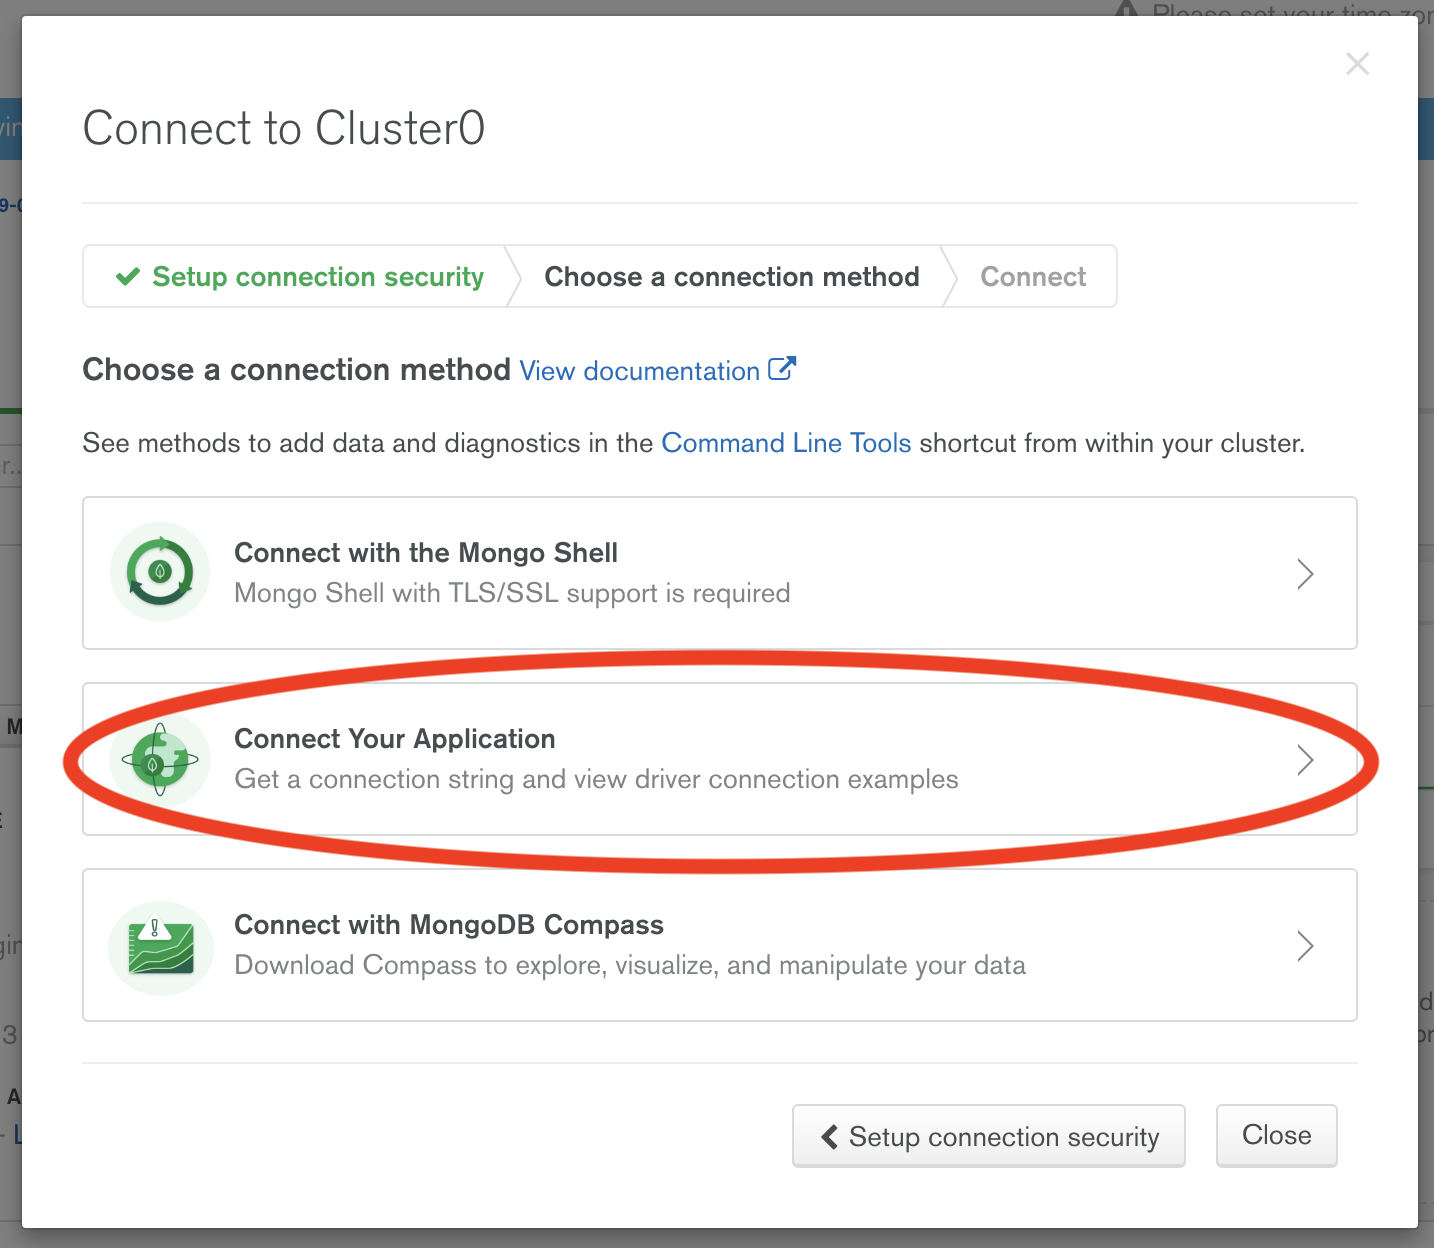
\includegraphics[width=14cm]{WEB/mongo_11.png}
    \end{center}
\end{figure}

\newpage
This is the address we will need for connecting to our database.
\begin{figure}[H]
    \begin{center}
        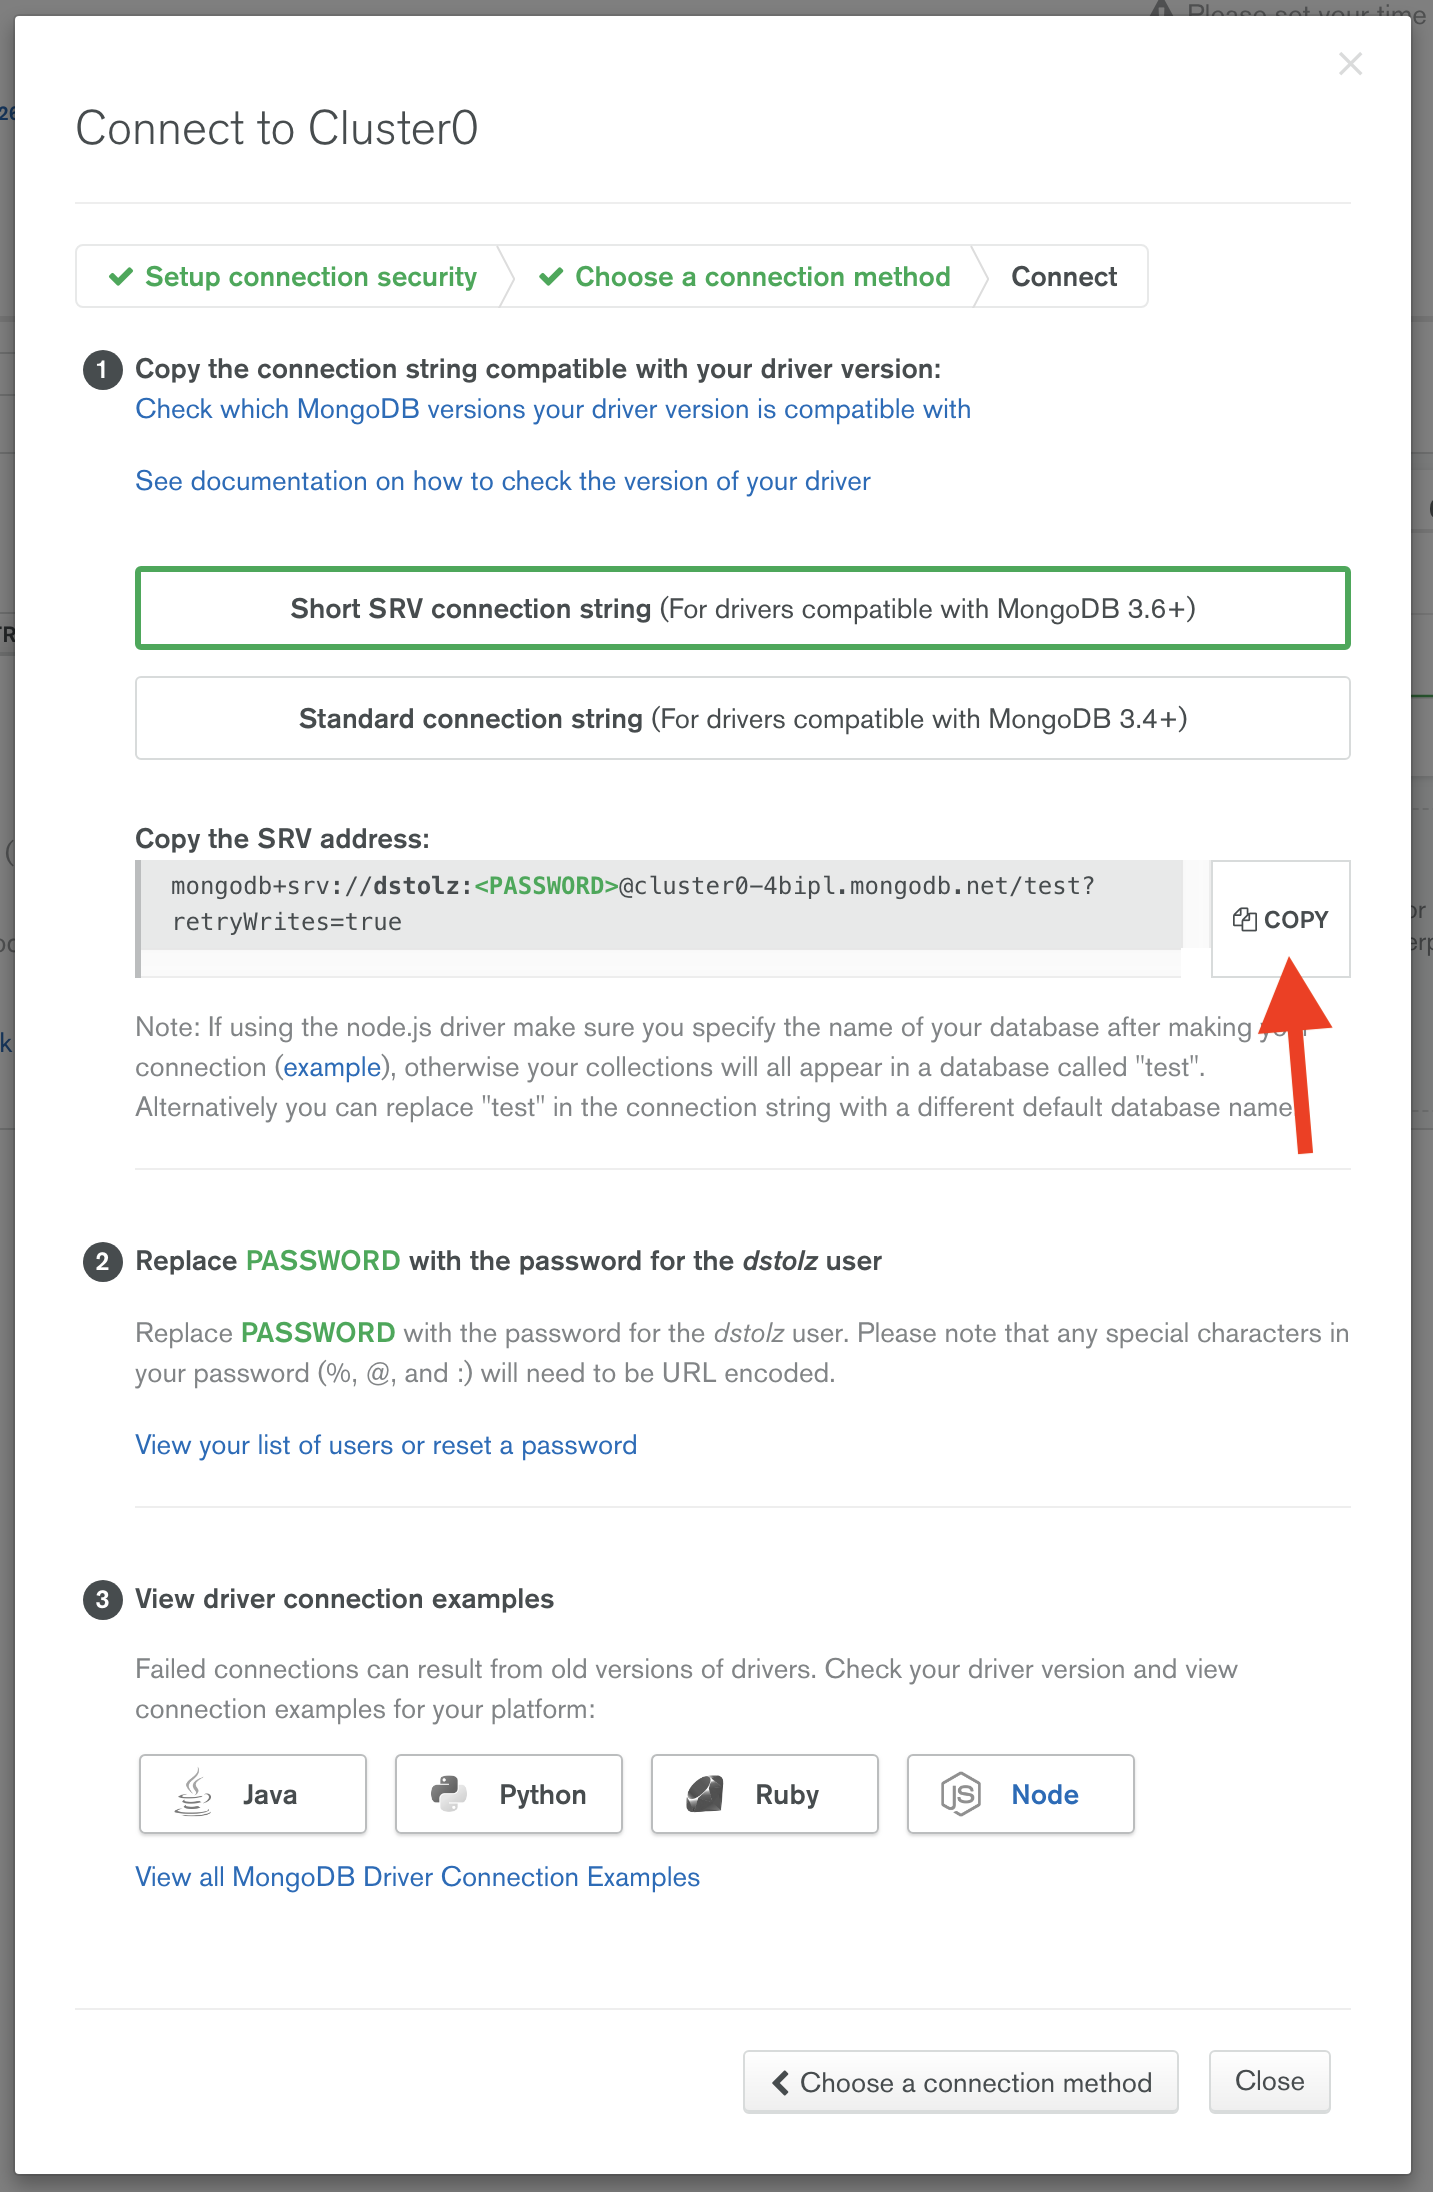
\includegraphics[width=14cm]{WEB/mongo_12.png}
    \end{center}
\end{figure}
That’s all for this project, but we will cover more MongoDB in the NodeJS course where you’ll be using MongoDB to store your todo list items.

%******************************************************************************%
\end{document}